\documentclass{article}
\usepackage{latexsym}
\usepackage{amssymb,amsmath,amsfonts}
\usepackage{custom2}
\usepackage{graphicx} 
\usepackage{epstopdf} 
\usepackage{caption}
\usepackage{subcaption}
\usepackage{url}
\usepackage[all,arc]{xy}
\usepackage{enumerate}
\usepackage{mathrsfs}
\usepackage{booktabs}
\usepackage[pdftex]{hyperref}
\usepackage{lscape}
\usepackage{xcolor}
\usepackage{natbib}
\usepackage{tabularx}
\newcommand{\tabitem}{~~\llap{\textbullet}~~}

\captionsetup{justification=RaggedRight, singlelinecheck=false}
\newcommand{\ra}[1]{\renewcommand{\arraystretch}{#1}}
\newcommand{\argmax}{\text{argmax}}
\newcommand{\Tr}{\text{Tr}}
\newcommand{\mb}{\mathbf}
\newtheorem{ass}{Assumption}

\addtolength{\evensidemargin}{-.5in}
\addtolength{\oddsidemargin}{-.5in}
\addtolength{\textwidth}{1.4in}
\addtolength{\textheight}{1.4in}
\addtolength{\topmargin}{-.5in}

\renewcommand{\thefigure}{S\arabic{figure}}
%\setcounter{figure}{0}  

\pagestyle{empty}

\title{Conflict and Strategy in Collective Computation}
\author{Eleanor Brush, David Krakauer, Jessica Flack}

\begin{document}
\maketitle
\tableofcontents


\section{Sequential Probability Ratio Test \label{SPRT}}
%The sequential probability ratio test (SPRT) 

In this section, we describe the the sequential probability ratio test (SPRT) and provide more details on why we chose to use a leaky integrator model (LIM) rather than an SPRT. The SPRT is a sequential hypothesis test. We are interested in testing the hypotheses $H_1:$ $Y$ is drawn from $p_1(y)$ and $H_2:$ $Y$ is drawn from $p_2(y)$. If we sample $Y$ repeatedly and observe the sequence $\{y_1,\dots,y_k\}$, then we form the decision variable $$Z_k=\sum_{i=1}^k\log\left(\frac{p_1(y_i)}{p_2(y_i)}\right).$$ The procedure dictated by the SPRT is to continue sampling until it happens that $Z_k>T_1$ or $Z_k<-T_2$, where $T_1$ and $T_2$ are thresholds determined by the desired error rate of the hypothesis test. If $Z_k>T_1$ first, then we accept $H_1$ and, if $Z_k<-T_2$, then we accept $H_2$.


The SPRT is the optimal way to decide between two alternatives in a noisy environment, in the sense that, for a given decision time, the SPRT is the most accurate algorithm and, for a given error rate, the SPRT reaches a decision most quickly \cite{Bogacz:2006uq,Froment:2010fk}.  The SPRT is mathematically equivalent to the LIM when the leak rate $\ell=0$ \cite{Bogacz:2006uq}. The LIM has the advantage over the SPRT of describing a more realistic leaky decision process and of being more analytically tractable.  While the SPRT has been applied to animal conflicts  \cite{Froment:2010fk}, to our knowledge the leaky integrator model has not been.

\section{Derivation of PDEs for decision time, error rate, and probability of reaching decision preference \label{pdes_deriv}}
In this section, we derive partial differential equations that describe the decision time, error rate, and probability of reaching decision preference for the LIM described in the main text. The derivation below follows closely that given in \cite{Gardiner:2009fk}, which provides more details.
For the sake of generality, we will write our system of stochastic differential equations as
\begin{equation*}
d{\mathbf x} ={\mb A}({\mb x},t)dt+{\mb B}({\mb x},t)d{\mb W}_t,% \label{sde}
\end{equation*}
where ${\mb x}\in\R^N$, $A:\R^N\times \R\to\R^N$, ${\mb B}:\R^N\times\R\to\R^N\times\R^N$, and ${\mb W}$ is an $N$-dimensional Wiener process. The forward equation describing the probability density $p({\mb x},t|{\mb y},s)$ is 
%% i'm trying to be consistent about my noise terms: I'll try to always use B*B^T even though Gardiner seems to switch back and forth between B and B*^T
\begin{equation}
\frac{\partial p}{\partial t} =-\sum_{i=1}^N\frac{\partial \big(A_i({\mb x},t)p\big)}{\partial x_i}+\frac{1}{2}\sum_{i,j=1}^N\frac{\partial^2\big([{\mb B}({\mb x},t){\mb B}^T({\mb x},t)]_{ij}p\big)}{\partial x_i\partial x_j} \label{forward}
\end{equation}
and the backward equation is 
\begin{equation}
-\frac{\partial p}{\partial s}=\sum_{i=1}^NA_i({\mb y},s)\frac{\partial p}{\partial y_i}+\frac{1}{2}\sum_{i,j=1}^N[{\mb B}({\mb y},s){\mb B}^T({\mb y},s)]_{ij}\frac{\partial^2 p}{\partial y_i\partial y_j}. \label{backward}
\end{equation}

\subsection{Decision time }
%(section 5.5 the Fokker-Planck Equation, First Passage Times for Homogeneous Processes in Gardiner) 
Let $G({\mathbf y},t)$ be the probability that the particle is still in a region $R$ at time $t$, given that it started at ${\mathbf y}$ so that $$G({\mathbf y},t)=\int_Rp({\mathbf x},t|{\mathbf y},0)d{\mathbf x}.$$  

\begin{claim} If the system is time homogeneous,
\begin{equation}
\frac{\partial G}{\partial t}=\sum_{i=1}^NA_i({\mb y})\frac{\partial G}{\partial y_i}+\frac{1}{2}\sum_{i,j=1}^N[{\mb B}({\mb y}){\mb B}^T({\mb y})]_{ij}\frac{\partial^2 G}{\partial y_i\partial y_j}. \label{Geq}
\end{equation}
%%Gardiner has a 2 instead of 1/2 in Section 6.6 but that must be a typo
\end{claim}
\begin{pf}
If the system is time homogeneous, then $p({\mb x},t|{\mb y},0)=p({\mb x},0|{\mb y},-t)$ so that we can rewrite $G$ as 
\begin{align*}
G({\mb y},t)&=\int_Rp({\mb x},0|{\mb y},-t)d{\mb x},
\\\Rightarrow \frac{\partial G}{\partial t}\bigg|_{t=t}&=\int_R\frac{\partial p({\mb x},0|{\mb y},-t)}{\partial t}\bigg|_{t=t}d{\mb x}
\\&=\int_R -\frac{\partial p({\mb x},0|{\mb y},s)}{\partial s}\bigg|_{s=t} d{\mb x}
\\&=\int_R\bigg(\sum_{i=1}^NA_i({\mb y})\frac{\partial p}{\partial y_{i}}\bigg|_{s=t}+\frac{1}{2}\sum_{i,j=1}^N[{\mb B}({\mb y}){\mb B}^T({\mb y})]_{ij}\frac{\partial^2 p}{\partial y_{i}\partial y_{j}}\bigg|_{s=t}\bigg) d{\mb x} \text{ using (\ref{backward})}
\\&=\sum_{i=1}^NA_i({\mb y})\bigg(\int_R\frac{\partial p}{\partial y_{i}}\bigg|_{s=t}d{\mb x}\bigg)+\frac{1}{2}\sum_{i,j=1}^N[{\mb B}({\mb y}){\mb B}^T({\mb y})]_{ij}\bigg(\int_R\frac{\partial^2 p}{\partial y_{i}\partial y_{j}}\bigg|_{s=t}\bigg) d{\mb x}
\\&=\sum_{i=1}^NA_i({\mb y})\frac{\partial G}{\partial y_i}+\frac{1}{2}\sum_{i,j=1}^N[{\mb B}({\mb y}){\mb B}^T({\mb y})]_{ij}\frac{\partial^2 G}{\partial y_i\partial y_j}
\end{align*}
\end{pf}

We can now use Equation (\ref{Geq}) to find an equation that the expected hitting time satisfies. If $T$ is the time at which the particle hits the boundary $S=\partial R$, then $P(T\geq t|{\mb y})=G({\mathbf y},t)$.  Therefore
\begin{align*}
E_{{\mathbf y}}(T) &=\int_0^\infty t P(T\in[t,t+dt)|{\mathbf y})
\\&= \int_0^\infty t \bigg(P(T\geq t|{\mathbf y})-P(T\geq t+dt|{\mathbf y})\bigg) 
\\&=\int_0^\infty t \bigg(G({\mathbf y},t)-G({\mathbf y},t+dt)\bigg)
\\&=\int_0^\infty t \frac{G({\mathbf y},t)-G({\mathbf y},t+dt)}{dt}dt
\\&=-\int_0^\infty t\frac{\partial G}{\partial t}dt
\\&=-\bigg(\big[tG({\mathbf y},t)\big]_0^{\infty}-\int_0^\infty G({\mathbf y},t)dt\bigg)  \text{ by integration by parts }
\\&=\int_0^\infty G({\mathbf y},t)dt \text{ if $\lim_{t\to \infty}G({\mathbf y},t)=0$ quickly enough}.
\end{align*}

If we let $f({\mathbf y})=E_{\mathbf y}(T)$, then 
\begin{align*}
\sum_{i=1}^NA_i({\mb y},t)\frac{\partial f}{\partial y_i}&+\frac{1}{2}\sum_{i,j=1}^N[{\mb B}({\mb y},t){\mb B}^T({\mb y},t)]_{ij}\frac{\partial^2 f}{\partial y_i\partial y_j}
\\&=\int_0^\infty\bigg(\sum_{i=1}^NA_i({\mb y},t)\frac{\partial G}{\partial y_i}+\frac{1}{2}\sum_{i,j=1}^N[{\mb B}({\mb y},t){\mb B}^T({\mb y},t)]_{ij}\frac{\partial^2 G}{\partial y_i\partial y_j}\bigg)dt
\\&=\int_0^\infty\frac{\partial G}{\partial t}dt \text{ using (\ref{Geq})}
\\&=G({\mb y},\infty)-G({\mb y},0)
\\&=-1
\end{align*}
Finally, this gives us a PDE for the expected hitting time of the boundary of the region $R$:
\begin{equation*}
\sum_{i=1}^NA_i({\mb y})\frac{\partial f}{\partial y_i}+\frac{1}{2}\sum_{i,j=1}^N[{\mb B}({\mb y}){\mb B}^T({\mb y})]_{ij}\frac{\partial^2 f}{\partial y_i\partial y_j}=-1% \label{DT}
\end{equation*}
with boundary conditions $f({\mb x})=0 \text{ for } {\mb x}\in\partial R$.

\subsection{Error rate }
%(section 6.6.2 The Fokker-Planck Equation in Several Dimensions, Distribution of Exit Points and section 5.5.4 Probability of Exit Through a Particular End of the Interval in Gardiner )
Let ${\mb J}({\mb x},t|{\mb y},s):(\R^N\times\R)\times(\R^N\times\R)\to \R^N$ be such that 
$$J_k({\mb x},t|{\mb y},s)=A_k({\mb x},t)p({\mb x},t|{\mb y},s)-\frac{1}{2}\sum_{l=1}^N\frac{\partial \big([{\mb B}({\mb x},t){\mb B}^T({\mb x},t)]_{kl}p({\mb x},t|{\mb y},s)\big)}{\partial x_j}.$$ 
If $p$ satisfies the forward equation (\ref{forward}), then 
\begin{equation}
\frac{\partial p}{\partial t} =-\sum_{i=1}^N\frac{\partial \big(A_i({\mb x},t)p\big)}{\partial x_i}+\frac{1}{2}\sum_{i,j=1}^N\frac{\partial^2\big([{\mb B}({\mb x},t){\mb B}^T({\mb x},t)]_{ij}p\big)}{\partial x_i\partial x_j}=-\sum_{i=1}^N\frac{\partial J_i({\mb x},t|{\mb y},s)}{\partial x_i}. \label{jequals}
\end{equation}
For this reason, $\mb{J}$ is called the probability current.

\begin{claim}
Each $J_k$  satisfies the backward equation.
\end{claim}
%\begin{landscape}
\begin{pf}
{\small
\begin{align*}
&\sum_{i=1}^NA_i({\mb y},s)\frac{\partial J_k({\mb x},t|{\mb y},s)}{\partial y_i}+\frac{1}{2}\sum_{i,j=1}^N[{\mb B}({\mb y},s){\mb B}^T({\mb y},s)]_{ij}\frac{\partial^2 J_k({\mb x},t|{\mb y},s)}{\partial y_i\partial y_j}
\\&=\sum_{i=1}^NA_i({\mb y},s)\bigg[A_k({\mb x},t)\frac{\partial p}{\partial y_i}-\frac{1}{2}\sum_{l=1}^N\frac{\partial \bigg([{\mb B}({\mb x},t){\mb B}^T({\mb x},t)]_{kl}\frac{\partial p({\mb x},t|{\mb y},s)}{\partial y_i}\bigg)}{\partial x_l}\bigg]
\\&+\frac{1}{2}\sum_{i,j=1}^N[{\mb B}({\mb y},s){\mb B}^T({\mb y},s)]_{ij}\bigg[A_k({\mb x},t)\frac{\partial^2 p}{\partial y_i\partial y_j}-\frac{1}{2}\sum_{l=1}^N\frac{\partial \bigg([{\mb B}({\mb x},t){\mb B}^T({\mb x},t)]_{kl}\frac{\partial^2 p({\mb x},t|{\mb y},s)}{\partial y_iy_j}\bigg)}{\partial x_l}\bigg]
\\&=A_k({\mb x},t)\bigg[\sum_{i=1}^NA_i({\mb y},s)\frac{\partial p}{\partial y_i}+\frac{1}{2}\sum_{i,j=1}^N[{\mb B}({\mb y},s){\mb B}^T({\mb y},s)]_{ij}\frac{\partial^2 p}{\partial y_i\partial y_j}\bigg]
\\&-\frac{1}{2}\sum_{l=1}^N\frac{\partial }{\partial x_l}\bigg([{\mb B}({\mb x},t){\mb B}^T({\mb x},t)]_{kl}\bigg[\sum_{i=1}^NA_i({\mb y},s)\frac{\partial p}{\partial y_i}+\frac{1}{2}\sum_{i,j=1}^N[{\mb B}({\mb y},s){\mb B}^T({\mb y},s)]_{ij}\frac{\partial^2 p}{\partial y_i\partial y_j}\bigg)\bigg]
\\&=A_k({\mb x},t)\bigg(-\frac{\partial p}{\partial s}\bigg)-\frac{1}{2}\sum_{l=1}^N\frac{\partial }{\partial x_l}\bigg(-[{\mb B}({\mb x},t){\mb B}^T({\mb x},t)]_{kl}\frac{\partial p}{\partial s}\bigg) \text{ using (\ref{backward})}
\\&=-\frac{\partial }{\partial s}\bigg(A_k({\mb x},t)p({\mb x},t|{\mb y},s)-\frac{1}{2}\sum_{l=1}^N\frac{\partial \big([{\mb B}({\mb x},t){\mb B}^T({\mb x},t)]_{kl}p({\mb x},t|{\mb y},s)\big)}{\partial x_l}\bigg)
\\&=-\frac{\partial J_k}{\partial s}.
\end{align*}
}
\end{pf}
%\end{landscape}

It follows that any linear combination $q({\mb x},t|{\mb y},s)=\sum_{k=1}^Nc_kJ_k({\mb x},t|{\mb y},s)$ also satisfies the backward equation:
\begin{equation}
-\frac{\partial q}{\partial s}=\sum_{i=1}^NA_i({\mb y},s)\frac{\partial q}{\partial y_i}+\frac{1}{2}\sum_{i,j=1}^N[{\mb B}({\mb y},s){\mb B}^T({\mb y},s)]_{ij}\frac{\partial ^2 q}{\partial y_i\partial y_j}. \label{jbackeq}
\end{equation}

\begin{claim} \label{probcurrent}
Consider two adjacent regions of space $R_1$ and $R_2$, where their shared boundary is denoted $S_{12}$. The net flow of probability from $R_2$ to $R_1$ can be written as $\int_{S_{12}} dS {\mb n}\cdot {\mb J}({\mb x},t) $ where ${\mb n}$ is a normal vector from $R_2$ to $R_1$.  
\end{claim}

\begin{pf}
Let $S_1$ be the part of the boundary of $R_1$ not shared with $R_2$ and $S_2$ be the part of the boundary of $R_2$ not shared with $R_1$ so that  $\partial R_1=S_1\cup S_{12}$, $R_2=S_2\cup S_{12}$, and $S_1\cap S_{12}=S_2\cap S_{12}=\emptyset$. The probability of crossing from $R_2$ to $R_1$ across $S_{12}$ in the interval of time $[t,t+dt)$ is 
\begin{align*}
\int_{R_1}d{\mb x}\int_{R_2}d{\mb y} p({\mb x},t+dt|{\mb y},t).
\end{align*}



The probability of crossing from $R_1$ to $R_2$ across $S_{12}$  in the interval of time $[t,t+dt)$ can be found analogously so the net flow $F$ from $R_2$ to $R_1$ at time $t$ is 
\begin{align*}
F=\lim_{dt \to 0}\frac{1}{dt}\int_{R_1}d{\mb x}\int_{R_2}d{\mb y} \big(p({\mb x},t+dt|{\mb y},t)-p({\mb y},t+dt|{\mb x},t)\big).
\end{align*}
Since $p({\mb x},t|{\mb y},t)=p({\mb y},t|{\mb x},t)=0$ for ${\mb y}\in R_2$ and ${\mb x}\in R_1$,
\begin{align*}
F&=\lim_{dt \to 0}\frac{1}{dt}\int_{R_1}d{\mb x}\int_{R_2}d{\mb y} \big(p({\mb x},t+dt|{\mb y},t)-p({\mb x},t|{\mb y},t)-p({\mb y},t+dt|{\mb x},t)+p({\mb y},t|{\mb x},t)\big)
\\&=\int_{R_1}d{\mb x}\int_{R_2}d{\mb y} \bigg(\frac{\partial p({\mb x},t'|{\mb y},t)}{\partial t'}\bigg|_{t'=t}-\frac{\partial p({\mb y},t'|{\mb x},t)}{\partial t'}\bigg|_{t'=t}\bigg)
\\&=\int_{R_1}d{\mb x}\int_{R_2}d{\mb y}\bigg(-\sum_{i=1}^N\frac{\partial J_i({\mb x},t|{\mb y},t)}{\partial x_i}+\sum_{i=1}^N\frac{\partial J_i({\mb y},t|{\mb x},t)}{\partial y_i}\bigg) \text{using (\ref{jequals})}
\\&=\int_{R_1}d{\mb x}\int_{R_2}d{\mb y}\sum_{i=1}^N\frac{\partial J_i({\mb y},t|{\mb x},t)}{\partial y_i}-\int_{R_2}d{\mb y}\int_{R_1}d{\mb x}\sum_{i=1}^N\frac{\partial J_i({\mb x},t|{\mb y},t)}{\partial x_i}
\\&=\int_{R_1}d{\mb x}\bigg[\int_{S_2}dS {\mb n_2}\cdot {\mb J}({\mb y},t|{\mb x},t)+\int_{S_{12}}dS {\mb n_2}\cdot {\mb J}({\mb y},t|{\mb x},t)\bigg]\\&-\int_{R_2}d{\mb y}\bigg[\int_{S_1}dS{\mb n}_1\cdot{\mb J}({\mb x},t|{\mb y},t)+\int_{S_{12}}dS{\mb n}_1\cdot{\mb J}({\mb x},t|{\mb y},t)\bigg]
\\&\text{ by the divergence theorem,}
\\ &\text{ where ${\mb n}_2$ is a normal pointing out of $R_2$ and similarly for ${\mb n}_1$.}
\end{align*}
For ${\mb y}\in S_2$ and ${\mb x}\in R_1$, $J({\mb y},t|{\mb x},t)=0$. Similarly, for ${\mb x}\in S_1$ and ${\mb y}\in R_2$, ${\mb J}({\mb x},t|{\mb y},t)=0$.  Therefore, the integrals over $S_2$ and $S_1$ disappear and $F$ simplifies to
\begin{align*}
F&=\int_{R_1}d{\mb x}\bigg[\int_{S_{12}}dS {\mb n_2}\cdot {\mb J}({\mb y},t|{\mb x},t)\bigg]-\int_{R_2}d{\mb y}\bigg[\int_{S_{12}}dS{\mb n}_1\cdot{\mb J}({\mb x},t|{\mb y},t)\bigg]
\\&=\int_{S_{12}}dS\bigg[\int_{R_1}d{\mb y}\ {\mb n}\cdot \mb{J}({\mb x},t|{\mb y},t)+\int_{R_2}d{\mb y}\ {\mb n}\cdot {\mb J}({\mb x},t|{\mb y},t)\bigg]
\\ & \text{ where ${\mb n}$ is a normal pointing from $R_2$ to $R_1$}
\\&=\int_{S_{12}}dS\bigg[\int_{R_1\cup R_2}d{\mb y}\ {\mb n}\cdot \mb{J}({\mb x},t|{\mb y},t)\bigg]
\\&=\int_{S_{12}}dS\ {\mb n}\cdot {\mb J}({\mb x},t).
% \text{ since $\mb{J}({\mb x},t|{\mb y},t)=\delta(\mb{x}=\mb{y})$}
%\\\text{ since ${\mb x}\in S_{12}\subset R_1\cup R_2$ and}
\end{align*}
\end{pf}

Now consider a region $R$ with boundary $S$.  Let $g({\mb a},{\mb x},t)|d{\mb S}({\mb a})|$ be the probability of exiting through an element $d{\mb S}({\mb a})$ of the boundary $S$ after time $t$.

\begin{claim}
If the system is time homogeneous, 
\begin{equation}
\frac{\partial g}{\partial t}=\sum_{i=1}^NA_i({\mb x})\frac{\partial g}{\partial x_i}+\frac{1}{2}\sum_{i,j=1}^N[{\mb B}({\mb x}){\mb B}^T({\mb x})]_{ij}\frac{\partial ^2 g}{\partial x_i\partial x_j}. \label{geq}
\end{equation}
\end{claim}

\begin{pf}
By the definition of $g$,
{
%% Gardiner has a negative sign in the following but I don't know why and it seems to work out just fine without it?
\begin{align*}
g({\mb a},{\mb x},t)|d{\mb S}({\mb a})|
&=\int_t^\infty dt' {\mb J}({\mb a},t'|{\mb x},0)\cdot d{\mb S}(\mb{a}) \text{ using Claim \ref{probcurrent}}
\\&=\int_t^\infty dt' {\mb J}({\mb a},0|{\mb x},-t')\cdot d{\mb S}(\mb{a})
\\&=\int_{-\infty}^{-t}dt' {\mb J}({\mb a},0|{\mb x},t')\cdot d{\mb S}(\mb{a})\\& \text{ using integration by substitution}
\\ \text{ so that }  \sum_{i=1}^NA_i({\mb x})\frac{\partial g}{\partial x_i}&+\frac{1}{2}\sum_{i,j=1}^N[{\mb B}({\mb x}){\mb B}^T({\mb x})]_{ij}\frac{\partial ^2 g}{\partial x_i\partial x_j}=
\\&\int_{-\infty}^{-t} dt'\bigg(\sum_{i=1}^NA_i({\mb x})\frac{\partial ({\mb J}({\mb a},0|{\mb x},t')\cdot d{\mb S}({\mb a}))}{\partial x_i}\\&+\frac{1}{2}\sum_{i,j=1}^N[{\mb B}({\mb x}){\mb B}^T({\mb x})]_{ij}\frac{\partial ^2 ({\mb J}({\mb a},0|{\mb x},t')\cdot d{\mb S}({\mb a}))}{\partial x_i\partial x_j}\bigg)
\\&=\int_{-\infty}^{-t}dt' \bigg(-\frac{\partial ({\mb J}({\mb a},0|{\mb x},t')\cdot d{\mb S}({\mb a}))}{\partial t'}\bigg) \text{ using Eq.  (\ref{jbackeq})}
\\&=\big(-{\mb J}({\mb a},0|{\mb x},t')\cdot d{\mb S}({\mb a})\big)\bigg|_{-\infty}^{-t}
\\&=\big(-{\mb J}({\mb a},-t'|{\mb x},0)\cdot d{\mb S}({\mb a})\big)\bigg|_{-\infty}^{-t}
\\&=-{\mb J}({\mb a},t|{\mb x},0)\cdot d{\mb S}({\mb a})\
\\&=\frac{\partial g}{\partial t}.
\end{align*}
}
\end{pf}

We are interested in finding the total probability of exiting through $d{\mb S}({\mb a})$, $h({\mb a},{\mb x})=g({\mb a},{\mb x},0)$.  In the course of the proof of the last claim, we found that
\begin{equation*}
\sum_{i=1}^NA_i({\mb x})\frac{\partial g({\mb a},{\mb x},t)}{\partial x_i}+\frac{1}{2}\sum_{i,j=1}^N[{\mb B}({\mb x}){\mb B}^T({\mb x})]_{ij}\frac{\partial ^2 g({\mb a},{\mb x},t)}{\partial x_i\partial x_j}=-{\mb J}({\mb a},t|{\mb x},0)\cdot d{\mb S}({\mb a}).
\end{equation*}
If we let $t\to 0$ and notice that ${\mb J}({\mb a},0|{\mb x},0)=\delta(|{\mb a}-{\mb x}|)$, we find that 
\begin{equation*}
\sum_{i=1}^NA_i({\mb x})\frac{\partial h}{\partial x_i}+\frac{1}{2}\sum_{i,j=1}^N[{\mb B}({\mb x}){\mb B}^T({\mb x})]_{ij}\frac{\partial ^2 h}{\partial x_i\partial x_j}=0
\end{equation*}
with boundary conditions $h({\mb a},{\mb x})=\delta(|{\mb a}-{\mb x}|)$ for ${\mb x}$ in $S$. To find the total probability of exiting through a section $S'\subset S$, $H(S',{\mb x})$, we can simply integrate the solutions $h({\mb a},{\mb x})$ for ${\mb a}\in S'$ to find 
\begin{equation*}
\sum_{i=1}^NA_i({\mb x})\frac{\partial H}{\partial x_i}+\frac{1}{2}\sum_{i,j=1}^N[{\mb B}({\mb x}){\mb B}^T({\mb x})]_{ij}\frac{\partial ^2 H}{\partial x_i\partial x_j}=0 %\label{ER}
\end{equation*}
with boundary conditions $H(S',{\mb x})=\delta({\mb x}\in S')$ for ${\mb x}\in S$.



%We can also consider the expected exit time, given that the particle exits through $d{\mb S}({\mb a})$, $T({\mb a},{\mb x})$:
%
%\begin{align*}
%T({\mb a},{\mb x})&=\int_0^\infty t P(\text{ exit in }[t,t+dt)|\text{ exit through }d{\mb S}({\mb a}))
%\\&=\int_0^\infty t\frac{P(\text{ exit through }d{\mb S}({\mb a}) \text{ in }[t,t+dt))}{P(\text{ exit through } d{\mb S}({\mb a}))}
%\\&=\frac{1}{{P(\text{ exit through } d{\mb S}({\mb a}))}}\int_0^\infty t P(\text{ exit through }d{\mb S}({\mb a}) \text{ in }[t,t+dt))
%\\&=\frac{1}{h({\mb a},{\mb x})}\int_0^\infty t\bigg(g({\mb a},{\mb x},t)-g({\mb a},{\mb x},t+dt)\bigg)
%\\&=\frac{1}{h({\mb a},{\mb x})}\int_0^\infty- t\frac{\partial g}{\partial t}dt
%\\&=-\frac{1}{h({\mb a},{\mb x})}\bigg([tg({\mb a},{\mb x},t)]_0^\infty-\int_0^\infty g({\mb a},{\mb x},t)dt\bigg) \text{ by integration by parts}
%\\&=\frac{1}{h({\mb a},{\mb x})}\int_0^\infty g({\mb a},{\mb x},t)dt \text{ if }\lim_{t\to\infty} g({\mb a},{\mb x},t)=0 \text{ quickly enough}
%\\\text{so that }T({\mb a},{\mb x})h({\mb a},{\mb x})&=\int_0^\infty g({\mb a},{\mb x},t)dt
%\end{align*}
%If we integrate (\ref{geq}) from $0$ to $\infty$ we find that 
%\begin{align*}
%-h({\mb a},{\mb x})=-g({\mb a},{\mb x},0)=\sum_{i=1}^NA_i({\mb x})\frac{\partial (Th)}{\partial x_i}+\frac{1}{2}\sum_{i,j=1}^N[{\mb B}({\mb x}){\mb B}^T({\mb x})]_{ij}\frac{\partial^2(Th)}{\partial x_i\partial x_j}.
%\end{align*}


\subsection{Our model }
We now introduce the operator ${\mb L}$ such that 
\begin{equation*}
{\mb L}(f)=\sum_{i=1}^NA_i({\mb x})\frac{\partial f}{\partial x_i}+\frac{1}{2}\sum_{i,j=1}^N[{\mb B}({\mb x}){\mb B}^T({\mb x})]_{ij}\frac{\partial ^2 f}{\partial x_i\partial x_j}. %\label{operator}
\end{equation*}
Then the expected time to hit the boundary $S$ satisfies ${\mb L}f=-1$ with boundary conditions $f({\mb x})=0$ for ${\mb x}\in S$ and the probability of hitting a subset $S'\subset S$ satisfies ${\mb L}H=0$ with boundary conditions $H({\mb x})=\delta({\mb x}\in S')$ for ${\mb x}\in S$.
The stochastic differential equations in our model are
\begin{equation*}
\begin{array}{ll}
dX_1&=\bigg(-\ell X_1(t)+br(2c-1)\bigg)dt+\bigg(b\sqrt{rc}\bigg)dW_{\text{A}t}-\bigg(b\sqrt{r(1-c)}\bigg)dW_{\text{B}t}
\\dX_2&=\bigg(-\ell X_2(t)-br(2c-1)\bigg)dt-\bigg(b\sqrt{rc}\bigg)dW_{\text{A}t}+\bigg(b\sqrt{r(1-c)}\bigg)dW_{\text{B}t},
\end{array}
\end{equation*}
This gives 
\begin{equation*}
{\mb A}({\mb x},t)=\left(\begin{array}{ll} 
-\ell x_1+br(2c-1)
\\ -\ell x_2-br(2c-1)
\end{array}\right), \text{ and }
\end{equation*}

\begin{equation*}
{\mb B}({\mb x},t)=\left(\begin{array}{ll} 
b\sqrt{rc} & -b\sqrt{r(1-c)}
\\ -b\sqrt{rc} & b\sqrt{r(1-c)}
\end{array}\right), \text{ so that }
\end{equation*}

\begin{equation*}
{\mb B}({\mb x},t){\mb B}^T({\mb x},t)
=\left(\begin{array}{ll}
b^2r & b^2r
\\ b^2r & b^2r
\end{array}\right)
\end{equation*}
Thus, the operator ${\mb L}$ is given by
\begin{align*}
%\begin{array}{ll}
{\mb L}(f)&=(-\ell x_1+br(2c-1))\frac{\partial f}{\partial x_1}+(-\ell x_2-br(2c-1))\frac{\partial f}{\partial x_2}\\&\ \ \ \ \ \ \ \ +\frac{1}{2}b^2r\frac{\partial^2 f}{\partial x_1^2}+\frac{1}{2}b^2r\frac{\partial^2 f}{\partial x_1\partial x_2}+\frac{1}{2}b^2r\frac{\partial^2 f}{\partial x_2\partial x_1}+\frac{1}{2}b^2r\frac{\partial^2 f}{\partial x_2^2} \notag
\\&=(-\ell x_1+br(2c-1))\frac{\partial f}{\partial x_1}+(-\ell x_2-br(2c-1))\frac{\partial f}{\partial x_2}\\&\ \ \ \ \ \ \ \ +b^2r\bigg(\frac{1}{2}\frac{\partial^2 f}{\partial x_1^2}+\frac{\partial^2 f}{\partial x_1\partial x_2}+\frac{1}{2}\frac{\partial^2 f}{\partial x_2^2} \bigg)
%\end{array}
\end{align*}
The region we are interested in is the one in which both individuals' opinions $(x_1,x_2)$ are greater than or equal to their respective thresholds, i.e. $$R=\{(x_1,x_2): x_1\geq -T_1 \text{ and } x_2\geq -T_2\}$$ so that $S=\partial R=\{(x_1,-T_2): x_1>-T_1\}\cup\{(-T_1,x_2):x_2>-T_2\}$.  The subset of the boundary we are interested in is the one that indicates a correct decision has been made, i.e. $x_2=-T_2$, so that $S'=\{(x_1,-T_2):x_1>-T_1\}$. The expected decision time is the expected hitting time of $S$. The probability of a correct decision is the probability of exiting $R$ through $S'$. The first component prefers that the second component reaches its threshold first, so the probability of reaching its decision preference is the same as the probability of a correct decision. The probability of reaching the decision preference of the second component is $1$ minus that probability.

There are analytical solutions to these equations when the system of SDEs is reduced to one dimension. However, we were not able to find an analytical solution for the full two-dimensional system and we therefore used numerical methods to solve the PDEs in this case. In order to  numerically solve the PDEs for decision time and error rate, we artificially close the region $R$ so that we can impose boundary conditions on a finite subset of the plane. In order to this, we pick two upper bounds $B_1$ and $B_2$ and restrict $R$ to $$R_2=\{(x_1,x_2): x_1\in [-T_1,B_1] \text{ and } x_2\in[ -T_2,B_2]\},$$ with boundary $S_2$. The subset of the boundary we are interested in becomes 
$$S'_2=\{(x_1,-T_2):x_1\in [-T_1,B_1]\}\cup\{(B_1,x_2):x_2\in [-T_2,B_2]\}$$
The boundary condition $f({\mb x})=0$ for ${\mb x}\in S$ becomes $f({\mb x})=0$ for ${\mb x}\in S_2$ and the condition $H({\mb x})=\delta({\mb x}\in S')$ for ${\mb x}\in S$ becomes $H({\mb x})=\delta({\mb x}\in S'_2)$ for ${\mb x}\in S_2$.

\section{Application of model to neural systems \label{neural} }
In this section, we provide details on how the LIM has been applied to neural decision-making. The experimental paradigm the LIM is often applied to is one in which an experimental subject, usually a monkey, is shown a visual stimulus in which some dots are moving either left or right and the rest are flashing randomly. The LIM describes the firing rates of two neuronal populations, one of which fires in response to left motion and the other of which fires in response to right motion. Our derivation of the LIM for our model system could also be used to derive the LIM describing the firing rates of the two populations. Instead of wins and losses, the two types of inputs would be dots moving left and dots moving right. Instead of an asymmetry in fighting ability, $c$ would describe the coherence of the moving dots. In models of the firing rates of neuronal populations, there are usually two independent sources of noise affecting the two neuronal populations, whereas in our model there is a single source of noise affecting both decision variables. However, we could derive  independent sources of noise using the same framework. Table 2 summarizes the interpretation of the model in the two systems. The similarity in the two models highlights the similarities between the two systems.



\section{Dimensionality and initial conditions of the SDEs \label{dimension_initconds} }
%\label{dimensionality_comp}
In this section, we discuss the sensitivity of our model to the initial conditions and we show that the two-dimensional and one-dimensional decision processes are nearly equivalent. 
In our analyses, we assume that both decision variables start at $0$, i.e. $X_1(0)=X_2(0)=0$.  If a component were to have previous information, it might start with a different initial condition. In our model system, a monkey could gain information about another monkey by observing its fights against other opponents, without ever encountering it in a fight directly.  If the monkey has prior information that the other monkey has a higher fighting ability, it might start with its decision variable below $0$ and conversely if it has information that the other monkey has a lower fighting ability.  However, incorporating this  into our model would require additional assumptions about how observations affect the decision variables, so for simplicity we assume that both decision variables start at $0$.

Regardless of initial conditions, we can compare the error rate and decision time from a two-dimensional process and a one-dimensional process.  The two-dimensional process ends when $X_1<-T_1$ or $X_2<-T_2$, for given thresholds $T_1$ and $T_2$. If $Y=X_1-X_2$, the one-dimensional process ends when $Y>T_1$ or $Y<-T_2$, for (possibly different) thresholds $T_1$ and $T_2$.
If we let $Z=X_1+X_2$, then we can use our model to write down the dynamics of $Y$ and $Z$. Specifically, from the dynamics of $X_1$ and $X_2$,
\begin{equation*}
\begin{array}{ll}
dX_1&=\bigg(-\ell X_1(t)+br(2c-1)\bigg)dt+b\sqrt{r}dW_{t}
\\dX_2&=\bigg(-\ell X_2(t)-br(2c-1)\bigg)dt-b\sqrt{r}dW_{t},
\end{array}
\end{equation*}
we find that 
\begin{equation*}
\begin{array}{ll}
dY&=\bigg(-\ell Y+2br(2c-1)\bigg)dt+2b\sqrt{r}dW_{t}
\\dZ&=-\ell Zdt.
\end{array}
\end{equation*}
Since $X_1$ and $X_2$ experience the same noise with opposite signs, their sum $Z$ is described by a deterministic differential equation with solution $Z(t)=Z(0)\exp(-\ell t)$. With the initial conditions $X_1(0)=X_2(0)=0$, $Z(t)=0$ for all $t$ and the dynamics of $X_1$ and $X_2$ are entirely described by the dynamics of $Y$. Otherwise, $Y$ only gives one dimension of the dynamics of $(X_1,X_2)$. 

%If the decision thresholds, $T_1$ and $T_2$, are allowed to vary freely then any combination of error rate and decision time can be achieved for either the full two-dimensional model or the reduced one-dimensional model. Without any constraints, it is therefore difficult to compare the performance of the two models. 
 To make the processes directly comparable, we consider symmetric thresholds, i.e. $T_1=T_2$.
% , which is a constraint commonly applied in analyses of the reduced model (for example \cite{Bogacz:2006uq,Brown:2005fk,Feng:2009kl}).  
With this constraint, for a given level of difficulty $c$, error rate becomes a well-defined function of decision time. 
With the initial conditions $X_1(0)=X_2(0)=0$, $Y$ captures the full dynamics of $X_1$ and $X_2$. Accordingly, the error rate given by analyzing either the two-dimensional or the one-dimensional process are identical (Figure \ref{dimensionality}a). With initial conditions biased toward the incorrect decision (i.e. $c>0.5$ and $X_1(0)<X_2(0)$), the two-dimensional process actually makes a decision with slightly lower error rate for a given decision time (Figure \ref{dimensionality}b).  Conversely, with initial conditions biased toward the correct decision (i.e. $c>0.5$ and $X_1(0)>X_2(0)$), the two-dimensional process makes a decision with slightly higher error rate for a given decision time (Figure \ref{dimensionality}c). However, the differences between the two processes are negligible and we use results from an analysis of the full two-dimensional process because it better describes our model system. 

The initial conditions affect the tradeoff between error rate and decision time, and therefore the absolute value of the Nash thresholds. To avoid including additional mechanisms in our model, we focus on the Nash thresholds when the initial conditions are not biased. However, we expect the Nash thresholds with bias toward the incorrect decision to respond similarly to how the Nash thresholds without bias respond to the optimization weights: they should increase when decision preference is more important and decrease when decision time is more important. The situation is slightly different if the initial conditions are biased toward the correct decision.  In this case, the pair can optimize both error rate and decision time by setting their thresholds low (Figure \ref{dimensionality}c).

\begin{figure}[tp]
\hspace{-1.75cm}
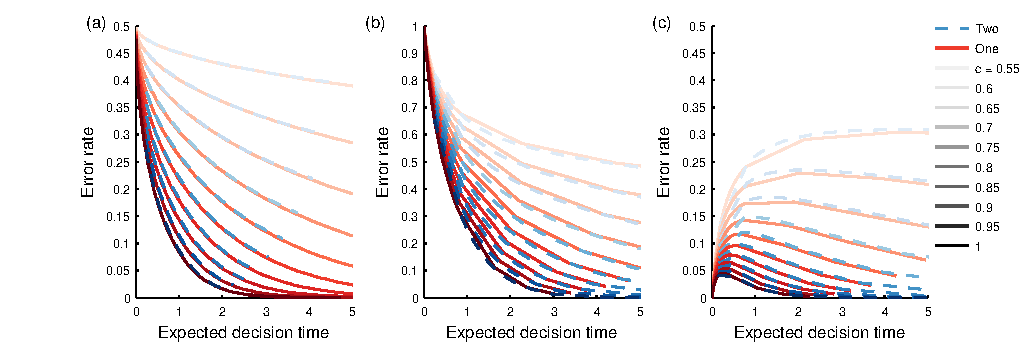
\includegraphics[width=6.9in]{dimensionality_comparison.pdf}
\caption{\label{dimensionality} The error rate decreases as decision time increases, as long as the initial conditions are not biased toward the correct decision. Here we show the probability of a correct output as a function of the expected time to a decision, as the decision thresholds are varied, with the constraint that $T_1=T_2$. The red lines correspond to the reduced one-dimensional model and the dashed blue lines correspond to the full two-dimensional process. Decisions of different difficulties ($c$) are represented with lines of different intensity. In (a), both decision variables start at $0$ and the two processes are equally accurate. In (b), $X_1(0)=1$, $X_2(0)=0.1$ (incorrect bias) and the two-dimensional process has a slightly lower error rate. In (c), $X_1(0)=0.1$, $X_2(0)=1$ (correct bias) and the two-dimensional process has a slightly higher error rate.  (Parameters: $N=20$, $b=1$, $r=1$, $\ell=0.1$.}
\end{figure}

%\appendix[Nash equilibrium]  
\section{Details on Nash equilibria \label{nash_supp}}
In this section, we discuss our procedure for finding the Nash equilibrium thresholds and how they might be reached in the model system. The Nash equilibrium thresholds are those such that no component can improve its utility by changing its threshold. The thresholds we allow in our model are $0.5,0.6,\dots,1.9,2$. To find the Nash thresholds, we assign all individuals in a group the highest possible strategy (although the procedure is robust to this choice of initial conditions). Each component, in turn, chooses the threshold that gives it the best utility, given the thresholds that the other components are using, until the components equilibrate on a set of Nash thresholds. If the Nash thresholds are $\{T_i\}$, there may be a set of thresholds $\{T_i'\}$ such that some components' utilities are better when the group uses the second set. However, no single individual has an incentive to change its strategy from $T_i$ to $T_i'$, and when the group uses the thresholds $\{T_i'\}$, at least one component will have an incentive to change its strategy. This sub-optimality is highlighted by our result that low-valued components would do better if all components raised their thresholds, even though no individual component has an incentive to do so. Our result agrees with previous findings that evolutionary dynamics of strategies for gathering social information can lead a population to use suboptimal strategies \cite{Torney:2015fk}.  By assuming that the components use Nash strategies, we are able to analyze the effects of the optimization weights, but we do not address the interesting question of how those strategies might be reached. Finding the appropriate timescale separation between the dynamics of how strategies are learned and the decision dynamics, and the consequences of this additional level of learning, are left for future work. 

\section{Calculation of mutual information \label{mut_info_calc} }
In this section, we explain how we calculate the mutual information between each measure of consensus and the underlying fighting abilities. 
%To evaluate the performance of each of our measures of consensus, we find the mutual information between scores given by each measure and underlying values or abilities.  
As explained in the main text and illustrated in Figure \ref{cartoon}, to generate a signaling network, we first draw a set of $N$ values $\{a_1,\dots,a_N\}$ from a uniform distribution. Then we find the Nash thresholds $\{T_1,\dots,T_N\}$, and then we find the expected decision times and probabilities of the decision outcomes for each pair of individuals. We then form an edge between each pair according to these probabilities, with a weight that depends on the decision time.  Once we have this signaling network, we apply each of our four consensus measures to it, generating consensus scores $\{s_1,\dots,s_N\}$.  To measure how well each measure performs, we find the mutual information between the consensus scores and the values. The mutual information between two random variables $X$ and $Y$ is 
\begin{equation}
I(X,Y)=\int_{y}\int_{x}p(x,y)\log\left(\frac{p(x,y)}{p(x)p(y)}\right)
\end{equation}
where $p(x,y)$ is the joint probability of $X$ and $Y$ and $p(x)$ and $p(y)$ are the marginal probabilities of $X$ and $Y$ respectively. For us, this becomes,
\begin{equation}
I(\{a_i\},\{s_i\})=\int_{\{a_i\}\in[0,1]^N}\int_{\{s_i\}\in\R^N}p(\{a_i\},\{s_i\})\log\left(\frac{p(\{a_i\},\{s_i\})}{p(\{a_i\})p(\{s_i\})}\right).
\end{equation}
If a measure produces consensus scores with high mutual information between the scores and the values, then knowing the consensus scores of the components in the system tells us (and possibly the components themselves) about the underlying values.  However, calculating the mutual information requires many more samples than are computationally feasible.  To reduce the number of states whose probabilities we want to evaluate, we discretize both the values and the scores.  Rather than trying to use the full set of consensus scores to infer the values, this is more like using the order of the consensus scores to infer the order of the values. Specifically, given a set of values $\{a_1,\dots,a_N\}$, we bin them into $10$ bins and assign each component a new value $a_i'\in\{1,\dots,10\}$ corresponding to the bin in which its value falls.  Similarly, given a set of consensus score $\{s_1,\dots,s_N\}$, we bin them into $10$ bins and assign each component a new score $s_i'\in\{1,\dots,10\}$ corresponding to the bin in which its score falls.  The mutual information between the discretized values and scores is
\begin{equation}
I(\{a_i'\},\{s_i'\})=\sum_{\{a_i'\}\in\{1,\dots,10\}^N}\sum_{\{s_i'\}\in\{1,\dots,10\}^N}p(\{a_i'\},\{s_i'\})\log\left(\frac{p(\{a_i'\},\{s_i'\})}{p(\{a_i'\})p(\{s_i'\})}\right).
\end{equation}

\section{Explanation for most informative measures of consensus \label{info_exp}}
In this section, we provide further explanation for why different measures of consensus are most informative with different optimization weights. 
Which measure is the most informative about the individuals' true values depends on how accurately pairwise decisions tend to be and what kind of errors are most frequent. When the error rate is quite low ($w_2<0.4$), the finer measures of consensus---weighted in-degree and eigenvector centrality---can use all of the information in the decision network to make fine distinctions between individuals, leading to consensus scores that are more informative than those from the coarser measures---in-degree and entropy.  Whether weighted in-degree or eigenvector centrality is more informative depends on what type of error is common. When there are no waiting costs ($w_2=0$) and the individuals value their personal preferences over error rate ($w_1<0.8$), low-valued individuals can sometimes wait out higher valued individuals, leading to an incorrect  decision being made in favor of a low individual at the expense of a high individual. Since eigenvector centrality takes the identity of the source of decisions into account, it will incorrectly assign the low individual a high score, whereas weighted in-degree will ignore the source and assign the low individual an appropriately low score.  Therefore, in these circumstances, weighted in-degree is more informative. When error rate matters ($w_1\geq 0.8$, $w_2=0$) or when there are low non-zero waiting costs ($0<w_2\leq 0.3$) low-valued individuals are less likely to wait out high-valued individuals, but there are a moderate amount of mistakes between pairs of individuals in the middle and bottom of the group. Consider two intermediate-valued individuals, with $A$ having slightly higher value than $B$. Another individual might make a mistake with respect to $B$ so that weighted in-degree gives $B$ a slightly higher score than $A$. But $A$ and $B$ will mostly decide correctly so that, despite errors, $B$ will tend to send more decisions than $A$. Since eigenvector centrality is affected by the decisions sent as well as received, it will correctly give $A$ a higher score. Therefore, in these circumstances, eigenvector centrality is the most informative. As waiting costs increase ($0.4 \leq w_2 \leq 0.5$) and decisions become even less accurate, even the high-valued individuals start to make mistakes. Now consider two high- valued individuals, with $A$ having slight higher value than $B$. If $A$ errs and decides strongly in favor of a lower value individual, eigenvector centrality will give $A$ a lower score because of those sent decisions and weighted in-degree will give $A$ a lower score because of the decisions it has prevented itself from receiving. However, $A$ is likely to make at most one more mistake than $B$ so that the number of individuals deciding in favor of either will be the same. Thus the coarseness of unweighted in-degree becomes an advantage by allowing it to group high-valued individuals together when finer measures would make incorrect fine distinctions. When decisions are even less accurate ($0.5<w_2<0.7$), weighted in-degree, unweighted in-degree, and eigenvector centrality can all get confused by incorrect decisions between any pair of individuals. What becomes especially difficult is distinguishing between low-value individuals, one of whom might incorrectly receive decisions from higher individuals. If a low-value individual receives correct decisions, they will be of similar strengths from even lower individuals. However, if it receives decisions from a higher individual, even though its score from any of the other measures will be increased, entropy decreases its score because of the difference in the strengths of signals coming from different types of individuals. In these circumstances, entropy does well at measuring the lack of consensus of decisions with respect of low individuals. When decisions are very inaccurate ($w_2>0.6$), weighted in-degree becomes the most reliable.
 
 
% \appendix[Skewness of DSP]
\section{Explanation of skewness being maximized at intermediate waiting costs\label{skewness_dets}}
In this section, we provide further explanation for why the skewness of the consensus scores is maximized at intermediate waiting costs. When waiting costs are low and accuracy is high, the decisions accurately represent the individuals' true  abilities, so the distribution of number of signalers accurately represents the distribution of abilities, which is not very right-skewed.  When waiting costs are high, decisions are so noisy that all individuals receive a similar number of decisions, giving a distribution that is quite uniform and not right-skewed.  At intermediate waiting costs, the decisions between individuals with low to intermediate values are very noisy, so that the individuals in the bottom and middle of the group receive a similar number of signals, but all individuals make accurate decisions with the top few individuals, which gives them high scores and results in a right-skewed distribution.

\section{Skewness of DSP across species \label{species}}
In this section, we explain how our model could explain differences in the DSP across species of macaques.
Different species of macaque have stereotypical power structures with different amounts of skewness \cite{Flack:2004oq,Preuschoft:2004ly,Waal:1985fk,Thierry:2000ij}.  One explanation might be that the distribution of fighting abilities is different from species to species, for instance if there is more or less variation in body size.  However, our model suggests that even if the underlying distribution of fighting abilities are identical, the priorities given to preference, error rate, and waiting costs can affect the distribution of power.  The benefit of having a partner agree to be subordinate, the benefit of reaching the ``correct" agreement, and the costs of fighting may vary from species to species, causing variation in the shape of the power structure.

%\pagebreak
\section{Supplemental figures }


\begin{figure}[bp]
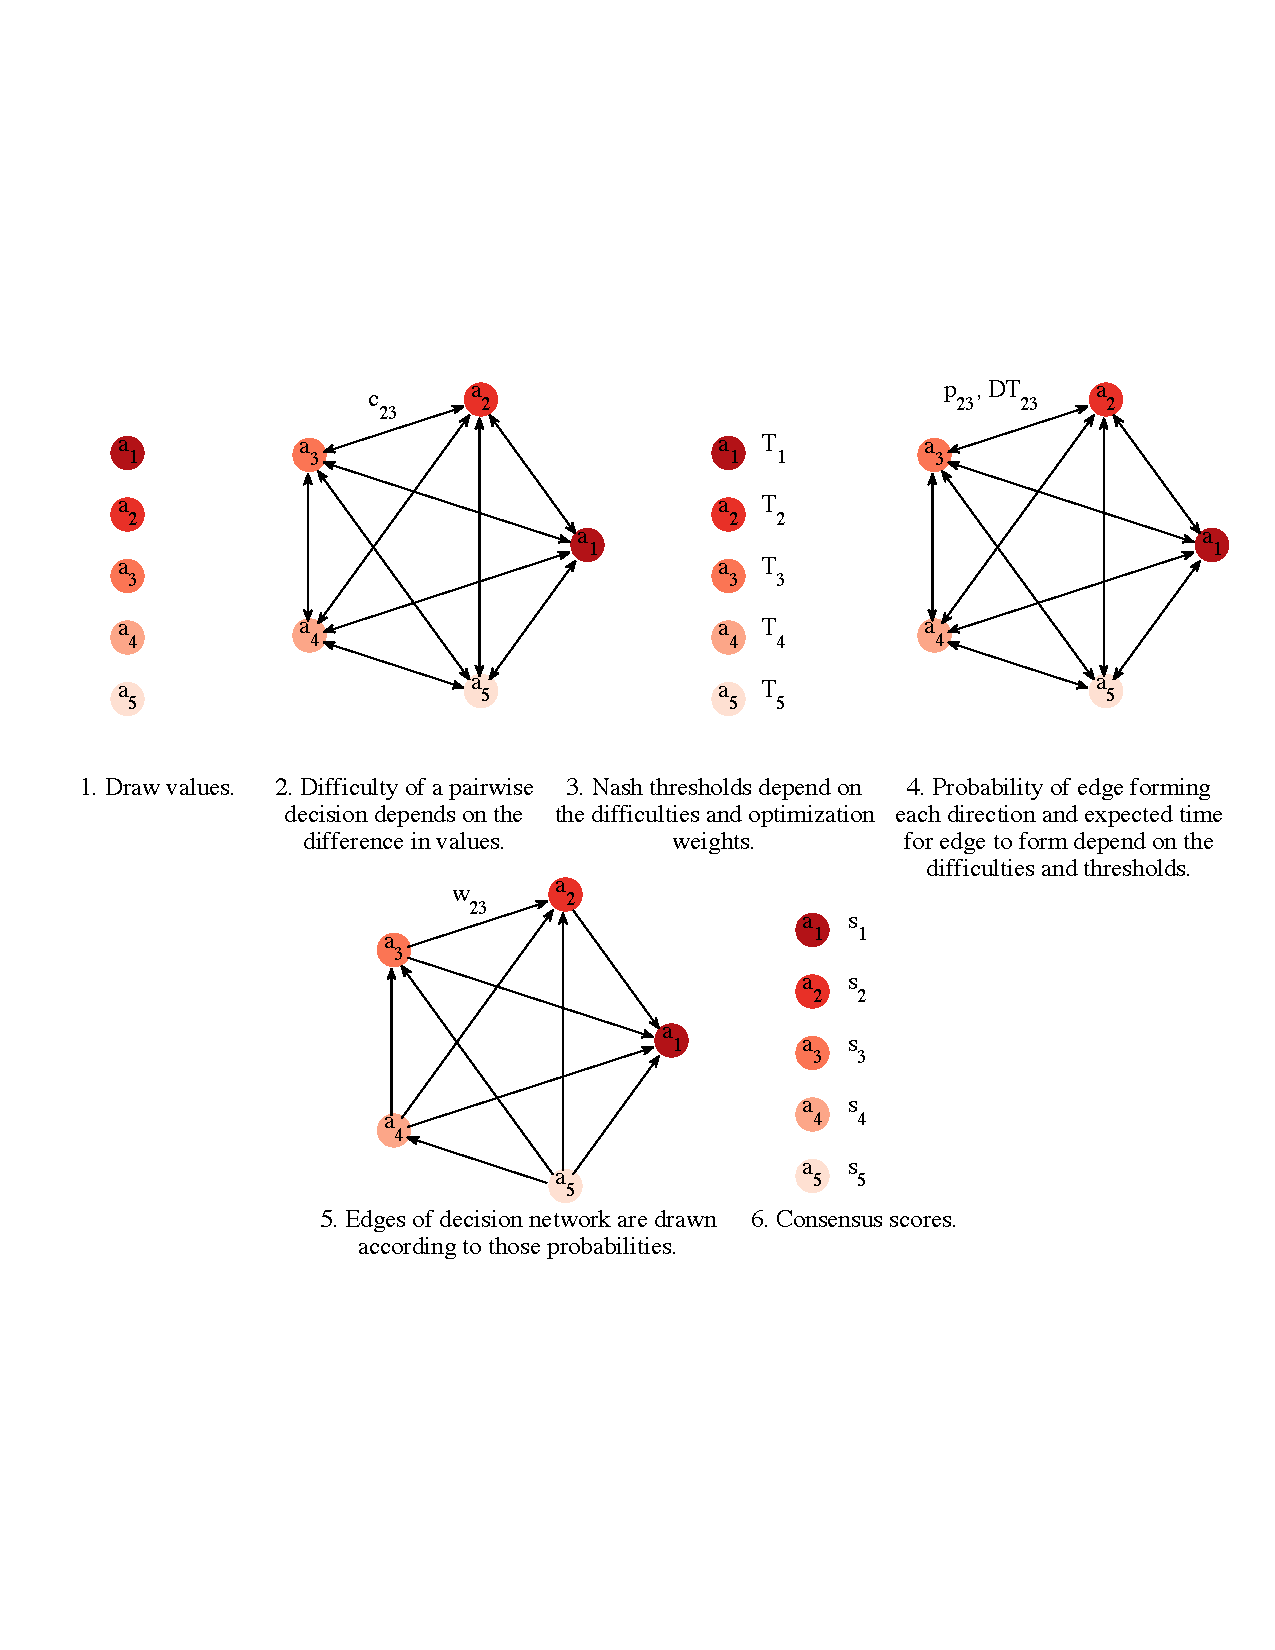
\includegraphics[width=6.83in]{cartoon_cropped.pdf}
\caption{\label{cartoon} Schematic of the model. 1. First, each individual's value is drawn from a uniform distribution. 2. The difficulty of each pairwise decision increases with the similarity of values, so that $c_{ij}$ increases as $|a_i-a_j|$ increases. 3. Given these difficulties, each individual has a Nash threshold strategy $T_i$. 4. Given the set of Nash thresholds, a pair will reach each decision with some probability and in an expected amount of time. 5. We draw the direction of each edge according to the probabilities of the two possible outcomes; the strength of the decision decreases with increasing decision time. 6. We apply a set of measures of consensus to each decision network, giving each individual a consensus score. We repeat this process for many random draws of values to find average Nash thresholds and the mutual information between the consensus scores and the values. }
\end{figure}

\begin{figure}[ht]
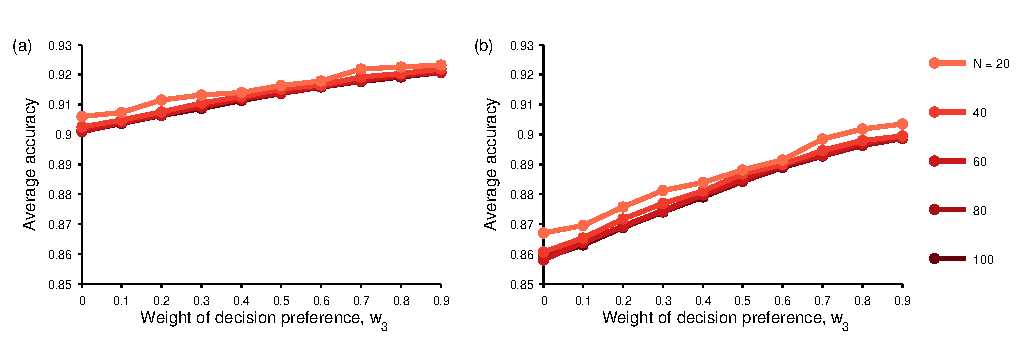
\includegraphics[width=6.83in]{group_size.pdf}
\caption{\label{groupsize} Increasing the weight given to decision preference improves the average error rate, regardless of the size of the group.  In each panel, the weight given to decision preference, $w_3$, is on the horizontal axis and average error rate is on the vertical axis. In (a) we show the average error rate of the whole group, and in (b) we show the average error rate of decisions made by the bottom quartile. Each line corresponds to a different group size $N$. Parameters: $b=1$, $r=1$, $\ell=0.1$, $w_2=0.1$, $w_1=1-w_3$.}
\end{figure}

\begin{figure}[ht]
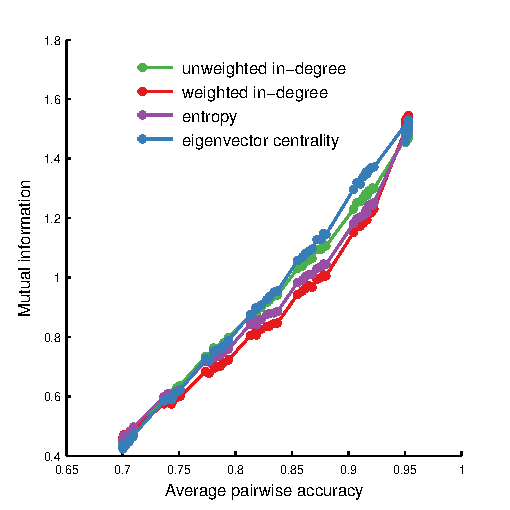
\includegraphics[width=3.4in]{mutinfo_vs_accuracy.pdf}
\caption{\label{mutinfo_vs_acc}  The mutual information of each consensus algorithm is a decreasing function of the average pairwise error rate.    This allows us to use average pairwise error rate as a proxy for the overall information content of the decision network, regardless of the algorithm being used. Parameters: $N=20$, $b=1$, $r=1$, $\ell=0.1$. }
\end{figure}

\begin{figure}[ht]
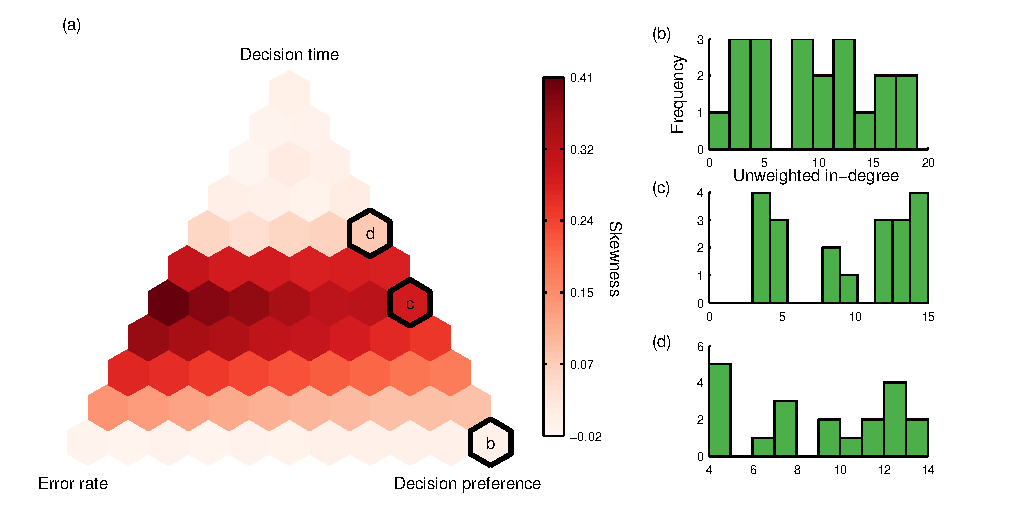
\includegraphics[width=6.83in]{skewness_histograms.pdf}
\caption{\label{histograms}  The average skewness of the distribution of unweighted in-degree is maximized at intermediate waiting costs. In (a), the color indicates the average skewness of the distribution of weighted in-degree for a group using Nash thresholds, as a function of the optimization weights, $w_1$, $w_2$, $w_3$. In the lower left corner of the simplex, only error rate matters ($w_1=1$).  In the upper corner, only decision time matters ($w_2=1$).  In the lower right corner, only preference matters ($w_3=1$).In (b)-(d) we show a histogram for a representative distribution of unweighted in-degree scores for a group using Nash thresholds. The optimization weights for each panel are indicated in the simplex with the corresponding letter.  Parameters: $w_1=0$, $w_2=0$, $w_3=1$ (c), $w_1=0$, $w_2=0.4$, $w_3=0.6$ (d), $w_1=0$, $w_2=0.6$, $w_3=0.4$ (e),  $N=20$, $b=1$, $r=1$, $\ell=0.1$.}
\end{figure}

\begin{figure}[ht]
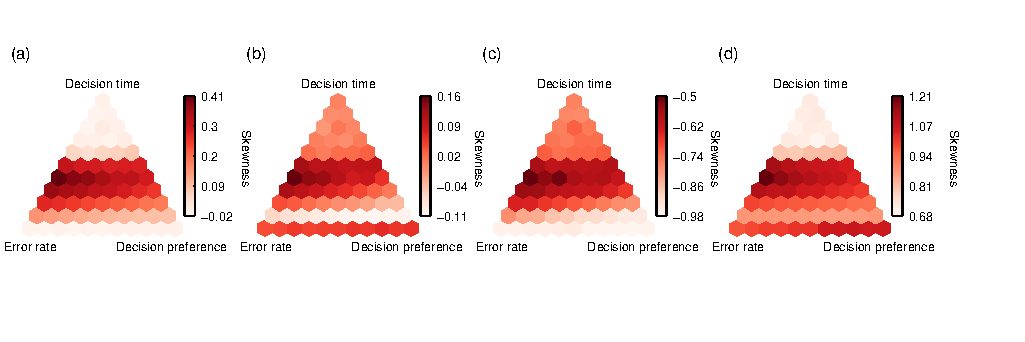
\includegraphics[width=6.83in]{multi_skewness.pdf}
\caption{\label{supp_skewness} The average skewness of the distribution of consensus scores from each measure is maximized at intermediate waiting costs.  In each panel, the color indicates the average skewness of the consensus scores of a group using Nash thresholds, as a function of the optimization weights, $w_1$, $w_2$, $w_3$. In the lower left corner of the simplex, only error rate matters ($w_1=1$).  In the upper corner, only decision time matters ($w_2=1$).  In the lower right corner, only preference matters ($w_3=1$). In (a) consensus is given by unweighted in-degree, in (b) by weighted in-degree, in (c) by entropy, and in (d) by eigenvector centrality. Parameters: $N=20$, $b=1$, $r=1$, $\ell=0.1$.} 
\end{figure}


\bibliographystyle{plain}
\bibliography{signaling_model}


\end{document}
